\section{Cooling Channel and Optics}
\label{Sect:CoolingChannel}

Having validated the diagnostics, it is now of interest to examine the properties
of the cooling channel.

\subsection{Input Beam}

The input beam distributions at the TKU reference planes are shown for position 
in fig. \ref{fig:tku_x} and \ref{fig:tku_y}, for transverse momentum in
fig. \ref{fig:tku_px} and \ref{fig:tku_py} and for total in momentum in
\ref{fig:tku_p}. The simulated beam and data show good agreement.

\begin{figure}[!tbh]
    \centering
    \topmatterallplots{03-Detectors}{compare_data}{tku_x}
    {Horizontal position distribution in TKU for all events in the upstream sample.}
\end{figure}

\begin{figure}[!tbh]
    \centering
    \topmatterallplots{03-Detectors}{compare_data}{tku_y}
    {Vertical position distribution in TKU for all events in the upstream sample.}
\end{figure}

\begin{figure}[!tbh]
    \centering
    \topmatterallplots{03-Detectors}{compare_data}{tku_px}
    {Horizontal momentum distribution in TKU for all events in the upstream sample.}
\end{figure}

\begin{figure}[!tbh]
    \centering
    \topmatterallplots{03-Detectors}{compare_data}{tku_py}
    {Vertical momentum distribution in TKU for all events in the upstream sample.}
\end{figure}

\begin{figure}[!tbh]
    \centering
    \topmatterallplots{03-Detectors}{compare_data}{tku_p}
    {Total momentum distribution in TKU for all events in the upstream sample.}
\end{figure}

\clearpage

\subsection{Magnets}

The MICE cooling channel consists of 12 coils arranged in 3 magnet assemblies, 
SSU, FC and SSD. As shown in fig. \ref{fig:hall_probes} the magnetic field 
is exceptionally reproducible, even over the several weeks over which the data
was taken.

\subsection{Beam Transport}

Bulk properties of the extrapolated beam are shown below. The measured points
show the beam extrapolated by the global track matching routines to various
z planes in the cooling channel geometry. The beam covariance matrix was 
calculated and various beam properties were drawn from the RMS ellipse. In the
following plots, blue points show properties of the upstream sample extrapolated from TKU
while red points show properties of the downstream sample extrapolated from TKD. The
extrapolation routines do not take into account stochastic processes such as
scattering, leading to a systematic discrepancy between the measured and 
extrapolated properties.

The 4-dimensional and 2-dimensional $\beta$ functions are shown in fig. 
\ref{fig:beta_4d}, \ref{fig:beta_x} and \ref{fig:beta_y}. The 2-dimensional 
$\beta$ functions are calculated using
\begin{equation}
\beta_{i} = Var(u_i) / \varepsilon_i
\end{equation}
where $Var(u_i)$ is the variance of either $x$ or $y$ and $\varepsilon_i$ is 
the corresponding 2-dimensional normalised RMS emittance. The 4-dimensional 
$\beta$ function is calculated using
\begin{equation}
\beta_{4d} = \frac{Var(x)+Var(y)}{2\varepsilon_{4d}}
\end{equation}
where $\varepsilon_{4d}$ is the 4-dimensional normalised RMS emittance.

Some $\beta$-beating is evident in TKU, especially in the 3-140 configuration.
This is expected; the Q789 triplet are not able to provide sufficient focussing
to reproduce the low $\beta$ functions required for adequate matching in SSU
without the additional scattering provided by the diffuser. The higher emittance
settings all reproduce similar optical performance. The 3-140 setting does 
yield a higher $\beta$ in the absorber leading to proportionately less cooling 
as per equation \ref{eq:depsdz}. The higher $\beta$ downstream of the focus
coil may be associated with optical emittance growth.

The momentum loss in the absorber does affect the beam behaviour downstream of 
the absorber. The lower momentum results in a stronger focusing affect and
larger phase advance, resulting in a focus (waist) in the region between M1D and
M2D.

\begin{figure}[!tbh]
    \centering
    \topmatterallplots{04-Cooling-Channel}{compare_optics}{beta_4d_ds}
    {$\beta_{4D}$ for events in the downstream sample, measured in TKU and 
    extrapolated downstream (blue points) and events in TKD extrapolated 
    downstream (red points). Red vertical lines indicate the position of ToF
    detectors, blue lines tracker stations and the green line represents the
    position of the absorber centre, when installed. \label{fig:beta_4d}} 
\end{figure}

\begin{figure}[!tbh]
    \centering
    \topmatterallplots{04-Cooling-Channel}{compare_optics}{beta_x_ds}
    {$\beta_{x}$ of events in the downstream sample, measured in TKU and 
     extrapolated downstream (blue points) and events in TKD extrapolated 
     downstream (red points). Red vertical lines indicate the position of ToF
    detectors, blue lines tracker stations and the green line represents the
    position of the absorber centre, when installed. \label{fig:beta_x}}
\end{figure}

\begin{figure}[!tbh]
    \centering
    \topmatterallplots{04-Cooling-Channel}{compare_optics}{beta_y_ds}
    {$\beta_{y}$ of events in the downstream sample, measured in TKU and 
     extrapolated downstream (blue points) and events in TKD extrapolated 
     downstream (red points). Red vertical lines indicate the position of ToF
    detectors, blue lines tracker stations and the green line represents the
    position of the absorber centre, when installed. \label{fig:beta_y}}
\end{figure}

The extrapolated RMS beam width is shown in fig. \ref{fig:sigma_x} and
\ref{fig:sigma_y}. The largest beam radius is just downstream of the absorber 
for all the configurations. There was a fixed mounting flange for the liquid 
Hydrogen absorber installed at this location, even when the absorber was not
installed. Interestingly, the 3 mm beam has 
rather a large beam radius owing to the beam transport issues outlined above.
This may result in transmission losses despite the smaller beam emittance.

\begin{figure}[!tbh]
    \centering
    \topmatterallplots{04-Cooling-Channel}{compare_optics}{sigma_0_ds}
   {Standard deviation of the vertical beam positions, $\sigma_{x}$, for events 
    in the downstream sample, measured in TKU and extrapolated downstream 
    (blue points) and events in TKD extrapolated downstream (red points). Red 
    vertical lines indicate the position of ToF detectors, blue lines tracker 
    stations and the green line represents the position of the absorber centre, 
    when installed. 
    \label{fig:sigma_x}}
\end{figure}

\begin{figure}[!tbh]
    \centering
    \topmatterallplots{04-Cooling-Channel}{compare_optics}{sigma_2_ds}
   {Standard deviation of the vertical beam positions, $\sigma_{y}$, for events 
    in the downstream sample, measured in TKU and extrapolated downstream (blue 
    points) and events in TKD extrapolated downstream (red points). Red 
    vertical lines indicate the position of ToF detectors, blue lines tracker 
    stations and the green line represents the position of the absorber centre, 
    when installed. 
    \label{fig:sigma_y}}
\end{figure}

\clearpage

\subsection{Absorber}

The main beam-based diagnostic of the absorber is the momentum loss of tracks
as they pass through it. Where tracks pass through thicker or more dense 
materials, they lose more energy.

The momentum change between trackers is shown as a function of the radius of
tracks extrapolated to the absorber midplane in fig. \ref{fig:dp_vs_r_abs}. For
the no absorber case there is a small momentum change arising
from the tracker Helium windows. When the lH2 windows were installed, there is
a significant tendency for higher radius tracks to lose more momentum, owing to
the thicker aluminium at higher radius. When the lH2 was filled, the higher
energy loss from aluminium appears to be offset due to the thickness of the
hydrogen itself. The momentum change in the lithium hydride is essentially
independent of radius, as expected from the cylindrical shape.

The momentum change in the absorber is shown as a function of the height of
tracks extrapolated to the absorber midplane in fig.  \ref{fig:dp_vs_y_abs}. 
There is no significant vertical correlation, beyond those noted above and the 
energy loss appears to be symmetric about the beamline.

\begin{figure}[!tbh]
    \centering
    \topmatterallplots{03-Detectors}{compare_data}{p_res_vs_global_through_virtual_absorber_centre_r_ds_cut}
    {Change in momentum between TKU and TKD as a function of the extrapolated
    track's distance from the beam axis at the absorber midplane. Vertical lines
    have been drawn at 0 and 20 MeV/c. \label{fig:dp_vs_r_abs}}
\end{figure}

\begin{figure}[!tbh]
    \centering
    \topmatterallplots{03-Detectors}{compare_data}{p_res_vs_global_through_virtual_absorber_centre_y_ds_cut}
    {Change in momentum between TKU and TKD as a function of the extrapolated
    track's height at the absorber midplane. Vertical lines
    have been drawn at 0 and 20 MeV/c. \label{fig:dp_vs_y_abs}}
\end{figure}

\begin{figure}[!tbh]
    \centering
    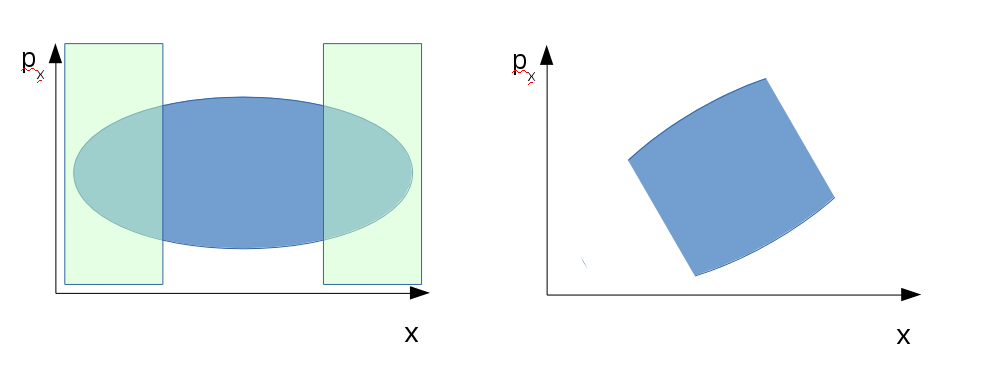
\includegraphics[width=0.8\textwidth]{04-Cooling-Channel/Figures/scraping_schematic.png}
    \caption{Schematic showing a beam ellipse scraped and then subsequently
    rotated in $(x, p_x)$ space by a focussing system. The resultant distribution
    will look quite non-Gaussian, potentially with the observed non-Gaussian 
    shoulders depending on the degree of rotation.\label{fig:scraping_schematic}}
\end{figure}

\subsection{Output Beam}
The position distribution of the downstream beam sample measured in TKD is shown 
in fig. \ref{fig:tkd_x} and fig. \ref{fig:tkd_y}. The 3-140 beam has significant 
shoulders. These can arise due to scraping, for example where the beam gets 
rather large around station 4 of TKD, as shown in \ref{fig:scraping_schematic}. 
The solenoid field between station 1 and
station 4 leads to a partial rotation of the region occupied by the scraped 
particles, both between horizontal and vertical spaces and between position and
momentum spaces. In general reasonable agreement is demonstrated between
simulation and data.

The transverse and total momenta in TKD is shown in fig. \ref{fig:tkd_px},
\ref{fig:tkd_py} and \ref{fig:tkd_p}. The transverse distributions are reproduced
in simulation with good agreement. The simulation shows more momentum loss than
the data; this was also observed in the momentum residual plot fig.
\ref{fig:tkd_extrapolated_p}. The additional momentum loss in simulation is
especially pronounced for the lithium hydride and empty absorber cases.


\begin{figure}[!tbh]
    \centering
    \topmatterallplots{03-Detectors}{compare_data}{tkd_x}
    {Horizontal position distribution in TKD for all events in the downstream sample.}
\end{figure}

\begin{figure}[!tbh]
    \centering
    \topmatterallplots{03-Detectors}{compare_data}{tkd_y}
    {Vertical position distribution in TKD for all events in the downstream sample.}
\end{figure}

\begin{figure}[!tbh]
    \centering
    \topmatterallplots{03-Detectors}{compare_data}{tkd_px}
    {Horizontal momentum distribution in TKD for all events in the downstream sample.}
\end{figure}

\begin{figure}[!tbh]
    \centering
    \topmatterallplots{03-Detectors}{compare_data}{tkd_py}
    {Vertical momentum distribution in TKD for all events in the downstream sample.}
\end{figure}

\begin{figure}[!tbh]
    \centering
    \topmatterallplots{03-Detectors}{compare_data}{tkd_p}
    {Total momentum distribution in TKD for all events in the downstream sample.}
\end{figure}

